\documentclass[tikz,border=2pt]{standalone}
\usepackage{amsmath,amssymb}
\usepackage{tikz}
\usetikzlibrary{arrows.meta}

\begin{document}
% From a story to an LP in five steps, illustrated with the Giapetto problem.
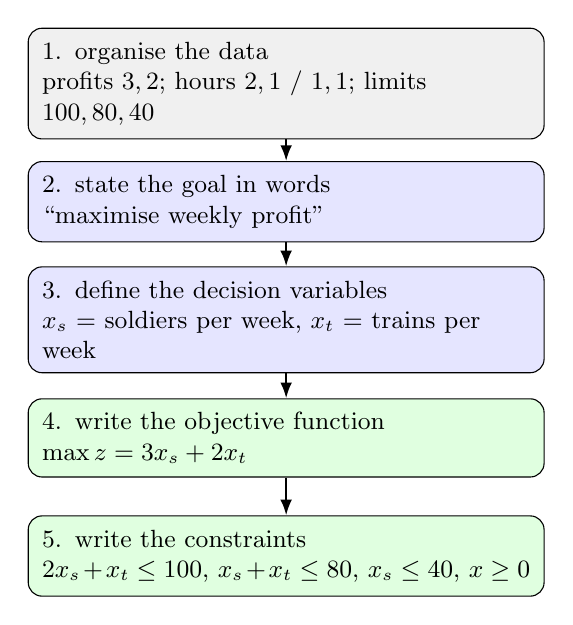
\begin{tikzpicture}[every node/.style={font=\small}, >={Latex[length=2mm]}, st/.style={draw, rounded corners=5pt, inner sep=5pt, align=left, text width=6.2cm}]
	\node[st, fill=gray!12] (s1) at (0,0) {1. organise the data\\ profits $3,2$; hours $2,1$ / $1,1$; limits $100,80,40$};
	\node[st, fill=blue!10] (s2) at (0,-1.5) {2. state the goal in words\\ ``maximise weekly profit''};
	\node[st, fill=blue!10] (s3) at (0,-3.0) {3. define the decision variables\\ $x_s$ = soldiers per week, $x_t$ = trains per week};
	\node[st, fill=green!12] (s4) at (0,-4.5) {4. write the objective function\\ $\max z=3x_s+2x_t$};
	\node[st, fill=green!12] (s5) at (0,-6.0) {5. write the constraints\\ $2x_s+x_t\le100$, $x_s+x_t\le80$, $x_s\le40$, $x\ge0$};
	\foreach \a/\b in {s1/s2, s2/s3, s3/s4, s4/s5} {\draw[->, thick] (\a) -- (\b);}
	\end{tikzpicture}
\end{document}
